\documentclass{article}
\usepackage{graphicx}
%\usepackage{varwidth}
%\usepackage{caption}
%\usepackage{float}
\usepackage{picinpar}
\begin{document}
%	this is dog picture
%	\begin{figure}
%		
\includegraphics[scale=0.4]{snuggle.jpg}
%		\caption{in plain format, if title too long, like normal paragraphics for display. 
%		if you set the formal small title,you can cut for paragraphics}
%	\end{figure}\par
%	this is cat type table
%	\begin{table}
%		\begin{tabular}{c|c|c}
%			name & sex & grade\\
%			\hline
%			lily & female & 6\\
%			lucy & female & 4\\
%			peter & male & 6\\
%		\end{tabular}
%		\caption{student information}
%	\end{table}\par
%	\begin{figure}
%		\centering
%		\begin{varwidth}[t]{\textwidth}
%			\vspace{0pt}
%			
\includegraphics[scale=0.2]{snuggle.jpg}
%		\end{varwidth}
%		\begin{varwidth}[t]{\textwidth}
%			\vspace{0pt}
%			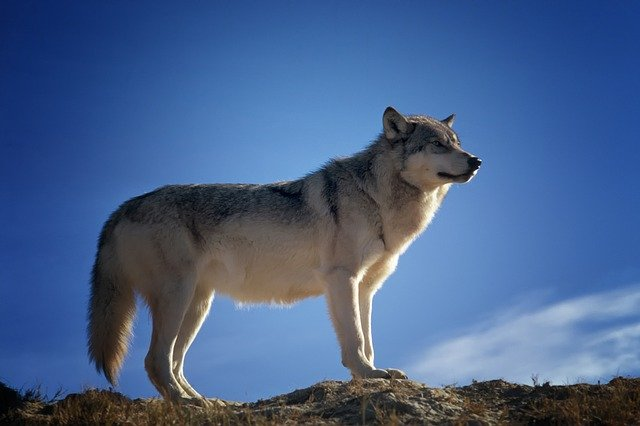
\includegraphics[scale=0.2]{wolf.jpg}
%		\end{varwidth}
%	\end{figure}

\begin{figwindow}[2,l,
	{
\includegraphics[width=8cm]{snuggle.jpg}},Lion]
	Alice was beginning to get very tired of sitting by her sister on the bank, and of having nothing to do: once or twice she had peeped into the book her sister was reading, but it had no pictures or conversations in it, ‘and what is the use of a book,’ thought Alice ‘without pictures or conversations?’

So she was considering in her own mind (as well as she could, for the hot day made her feel very sleepy and stupid), whether the pleasure of making a daisy-chain would be worth the trouble of getting up and picking the daisies, when suddenly a White Rabbit with pink eyes ran close by her.

There was nothing so very remarkable in that; nor did Alice think it so very much out of the way to hear the Rabbit say to itself, ‘Oh dear! Oh dear! I shall be late!’ (when she thought it over afterwards, it occurred to her that she ought to have wondered at this, but at the time it all seemed quite natural); but when the Rabbit actually took a watch out of its waistcoat-pocket, and looked at it, and then hurried on, Alice started to her feet, for it flashed across her mind that she had never before seen a rabbit with either a waistcoat-pocket, or a watch to take out of it, and burning with curiosity, she ran across the field after it, and fortunately was just in time to see it pop down a large rabbit-hole under the hedge.

In another moment down went Alice after it, never once considering how in the world she was to get out again.

The rabbit-hole went straight on like a tunnel for some way, and then dipped suddenly down, so suddenly that Alice had not a moment to think about stopping herself before she found herself falling down a very deep well.
\end{figwindow}

\end{document}


% begin{figure}...\end{figure}用于图片浮动体

% begin{table}...\end{table}用于表格浮动体

% 共同可选参数列表:
% h - 浮动体根据上下文顺序排列
% t - 浮动体排在当前页或下一页页首
% b - 浮动体排在当前页页尾
% p - 浮动体另外一页进行排列
% H - 不适用浮动体,不能与其他选项合用。包含在float宏包中
% 参数的优先级与顺序无关,通常按htbp顺序排列;当只有h参数时,拓展为ht参数集合;默认参数集合为tbp

% LaTeX最多同时保存18个未处理的浮动体

% \caption{string}为浮动体中的标题

% 在同一个浮动体中,表格和图标盒子可以并列排放。其中,表格按垂直方向居中对其,图片按垂直方向的基准线对齐

% \begin{varwidth}[t]{\textwidth}...\end{varwidth}用于确定宽度,\vspace{0pt}用于配置一个0pt空行,并按空行进行对齐
 
 % \begin{figwindow}[下降行数, 水平位置, 图内容, 图表题]...\end{figwindow}用于指定图片四周的文字绕排。包含在picinpar宏包中
 
 
 